Stadia is a new gaming platform by Google which is presented as the next evolution
of console gaming. The video gaming industry as it stands consists of several 
integral parts (as of now) one of which is the gaming console (Fig. \ref{fig:consoles}). The gaming 
console is the hardware necessary to experience video games. It can be expensive, 
hard to maintain and become irrelevant after several years of use (which requires 
purchasing a new console with new hardware).

\begin{figure}[H]
    \centering
    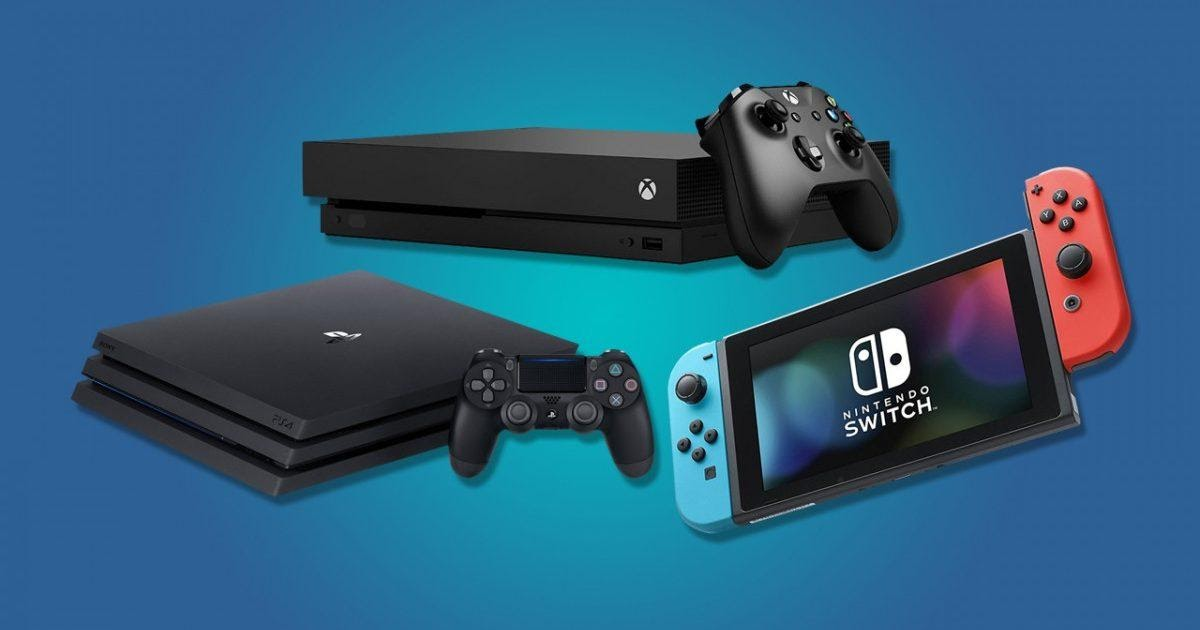
\includegraphics[width=10cm]{images/consoles.jpg}
    \caption{Gaming Consoles}
    \label{fig:consoles}
\end{figure}

Stadia tries to eliminate the console by offering video gaming as a subscription 
service like streaming services (Hulu, Netflix, etc...). with internet speed on the rise 
with the cloud computing industry taking shape, the possibility of removing the 
need of specialized hardware for gaming is increasing.
In this paper, we take a closer look on Stadia, what it does right, what is does wrong
and what can it do to achieve its goals.
